\documentclass[tikz]{standalone}

% color definitions
\usepackage{color}
\definecolor{A}{RGB}{255,71,71}
\definecolor{D}{RGB}{0,199,99}
\definecolor{C}{RGB}{36,145,255}
\definecolor{E}{RGB}{255,128,0}
\definecolor{Env}{RGB}{20, 210, 60}
\definecolor{Pheno}{RGB}{204, 204, 204}

\definecolor{Acol}{RGB}{255,71,71}
\definecolor{Dcol}{RGB}{0,199,99}
\definecolor{Ccol}{RGB}{36,145,255}
\definecolor{Ecol}{RGB}{255,128,0}

\newcommand{\colA}[1]{\textcolor{Acol}{#1}}
\newcommand{\colD}[1]{\textcolor{Dcol}{#1}}
\newcommand{\colC}[1]{\textcolor{Ccol}{#1}}
\newcommand{\colE}[1]{\textcolor{Ecol}{#1}}

\usepackage{pgf}
\usepackage{tikz}
\usepackage{pgfplots}
\usetikzlibrary{arrows}
\usetikzlibrary{matrix}
\usetikzlibrary{shapes}
\usetikzlibrary{fit}
\usetikzlibrary{positioning}
\usetikzlibrary{arrows.meta}
\usetikzlibrary{calc}
\tikzstyle{latent}=[circle, draw=black, thick]
\tikzstyle{manifest}=[rectangle, draw=black, thick, fill=white]
\tikzstyle{factor}=+[latent, fill=blue!20] 
\tikzstyle{A}=+[latent, fill=Acol, draw=Acol!30!black,text=Acol!30!black]
\tikzstyle{C}=+[latent, fill=Ccol, draw=Ccol!30!black,text=Ccol!30!black,opacity=0.3]
\tikzstyle{E}=+[latent, fill=Ecol, draw=Ecol!30!black,text=Ecol!30!black,opacity=0.2]
\tikzstyle{D}=+[latent, fill=Dcol, draw=Dcol!30!black,text=Dcol!30!black]
\tikzstyle{label}=[fill=white, circle, inner sep=1pt, minimum size=1pt] 
\tikzstyle{tiny label}+=[label, font=\scriptsize]
\tikzstyle{dub arrow1}=[shorten >= 2pt, shorten <= 2pt, dashed,line width=1.5,
transform canvas={shift={(-0.15,0)}}]
\tikzstyle{dub arrow2}=[shorten >= 2pt, shorten <= 2pt, dashed,line width=1.5,
transform canvas={shift={(0.15,0)}}] 
\tikzstyle{small node}=[scale=0.6]

\renewcommand{\familydefault}{\sfdefault}

\usepackage{blkarray}

\begin{document}
	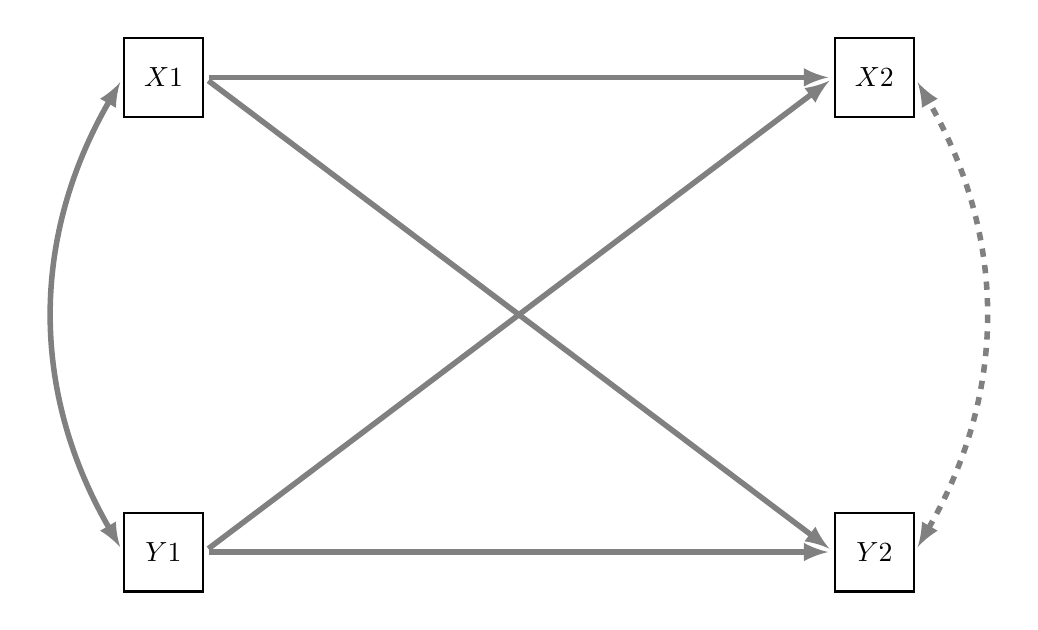
\begin{tikzpicture}[>=latex,node distance = 1.45 cm, minimum size = 1cm]
			\matrix[column sep = 8cm,row sep = 5cm]{
				\node (X11) at (0,0) [manifest] {$X1$}; &
				\node (X12) at (0,0) [manifest] {$X2$}; \\
				\node (X21) at (0,0) [manifest] {$Y1$}; &
				\node (X22) at (0,0) [manifest] {$Y2$}; \\
			};
			\path[->,shorten >= 2pt, shorten <= 2pt,line width=2,gray]
				(X11.east) edge (X12.west)
				(X11.east) edge (X22.west)
				(X21.east) edge (X22.west)
				(X21.east) edge (X12.west);
			\path[<->,shorten >= 2pt, shorten <= 2pt, bend left = 30, out = -30, in = -150, line width=2,gray]
				(X11.west) edge (X21.west)
				(X22.east) edge[dashed] (X12.east);
	\end{tikzpicture}

\[
V = \begin{blockarray}{*{5}{>{\scriptstyle\color{gray}}c}}
	& X1 & Y1 & X2 & Y2 \\
	\begin{block}{>{\scriptstyle\color{gray}}c(cccc))}
		X1 & V_{X1} & C_{X1, Y1} & C_{X1, X2} & C_{X1, Y2} \\
		Y1 & C_{Y1, X1} & V_{Y1} & C_{Y1, X2} & C_{Y1, Y2} \\
		X2 & C_{X2, X1} & C_{X2, Y1} & V_{X2} & C_{X2, Y2} \\
		Y2 & C_{Y2, X1} & C_{Y2, Y1} & C_{Y2, X2} & V_{Y2} \\
	\end{block}
	\end{blockarray}
\]

\[
V = (I - A)^{-1}S(I - A)^{-1T} = 
\begin{blockarray}
	
\end{blockarray}
\]

\end{document}